\section{RISC-V ISA}

RISC-V, which stands for the fifth generation of reduced instruction set computer, was first developed by Krste Asanović in 2010 at UC Berkeley.
Unlike ARM-based microprocessors, RISC-V is an open-source ISA. Hence, it has been considered "the Linux of microprocessors".
As a matter of fact, RISC-V is a lot more than that. The groundbreaking innovation lies in its modular design.

For a long time, incremental ISA, including x86 and ARM, has been the industry convention. In other words, architects keep adding instructions but never removing for the sake of backward compatibility.  
This leads to tremendous complexity in chip design. Besides, hardware costs increase since more silicon areas are required for decode and execution of a wider variety of instructions. And most importantly,
this monolithic design approach introduces less flexibility. There is the analogy - you pay for the whole buffet, but all you want is salad.

\subsection{RV32I Base Integer ISA}
RV32I is the most basic RISC-V ISA, where \texttt{32} indicates 32 bits wide registers and \texttt{I} stands for integer. There are 32 general purpose registers in RV32I, as shown in the upper part of table~\ref{table:riscv_register_calling_convention}. Among those registers, \texttt{x0} is hard-wired to 0, \texttt{x1} is used for holding return address, and \texttt{x10-x17} are used for function arguments.

As shown in fig~\ref{fig:riscv_base_instruction_format}, there are six types of instruction formats:

\begin{itemize}
    \item \textit{R-type} defines register-register operations. Its \texttt{opcode} is \texttt{0110011}. Operands are taken from registers \texttt{rs1} and \texttt{rs2} and result is written into register \texttt{rd}. Common R-type instructions are \texttt{add}, \texttt{sub}, \texttt{sll}, \texttt{slt}, \texttt{sltu}, \texttt{xor}, \texttt{srl}, \texttt{sra}, \texttt{or}, and \texttt{and}.
    
    \item \textit{I-type} defines register-immediate operations. Its \texttt{opcode} is \texttt{0010011}. The 12-bit immediate is sign extended to \texttt{word} and added with register \texttt{rs1}.
    Common I-type instructions are \texttt{addi}, \texttt{slti}, \texttt{sltiu}, \texttt{andi}, \texttt{ori}, and \texttt{xori}. In addition, load instructions, including \texttt{lw}, \texttt{lh}, \texttt{lhu}, \texttt{lb}, and \texttt{lbu}, are also I-type.
    
    \item \textit{S-type} defines store instructions, including \texttt{sb}, \texttt{sh}, and \texttt{sw}. Its \texttt{opcode} is \texttt{0100011}. Data stored in register \texttt{rs2} is stored into target memory address, which is calculated by adding base memory address in register \texttt{rs1} and immediate offset. Note that immediate is split into \texttt{imm[11:5]} and \texttt{imm[4:0]} due to design decision of keeping \texttt{rs1} and \texttt{rs2} in the same place as in R-type.
    
    \item \texttt{B-type} refers to branch instructions, including \texttt{beq}, \texttt{bne}, \texttt{blt}, \texttt{bge}, \texttt{bltu}, and \texttt{bgeu}. Its \texttt{opcode} is \texttt{1100011}. Registers \texttt{rs1} and \texttt{rs2} are compared with each other. If the branch is taken, the new \texttt{pc} is specified by the sum of current \texttt{pc} and \texttt{immediate}. Note that \texttt{imm[0]} is neglected since the RISC-V design specifies that branch offset is always multiples of 2 bytes.
    
    \item \texttt{U-type} refers to \texttt{lui} (load upper immediate) and \texttt{auipc} (add upper immediate to pc). \texttt{lui} deals with large immediate, which I-type instructions cannot handle. For example, in order to load \texttt{0x578ab111} into \texttt{x12}, the two steps are \texttt{lui x12, 0x578ab}, which loads \texttt{0x578ab} into the upper 20 bits and clears the lower 12 bits to 0, then \texttt{add x12, x12, 0x111}.
    
    \item \texttt{J-type} refers to unconditional jump instruction \texttt{jal} (jump and link). Target address is from adding immediate and current \texttt{pc}. Furthermore, since immediate is 21 bits, it can jump to any 16-bit aligned address \texttt{$\pm$1 MB} relative to current \texttt{pc}.
\end{itemize}

\begin{table}
    \centering
    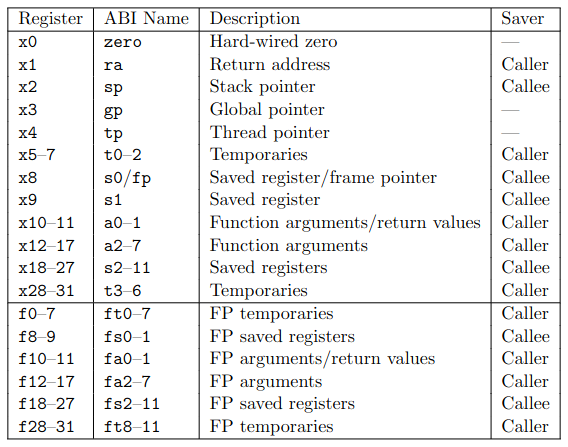
\includegraphics[width=.85\linewidth]{figures/RISCV_register_calling_convention.png}
    \caption{RISC-V register calling convention}
    \label{table:riscv_register_calling_convention}
\end{table}

\begin{figure}
    \centering
    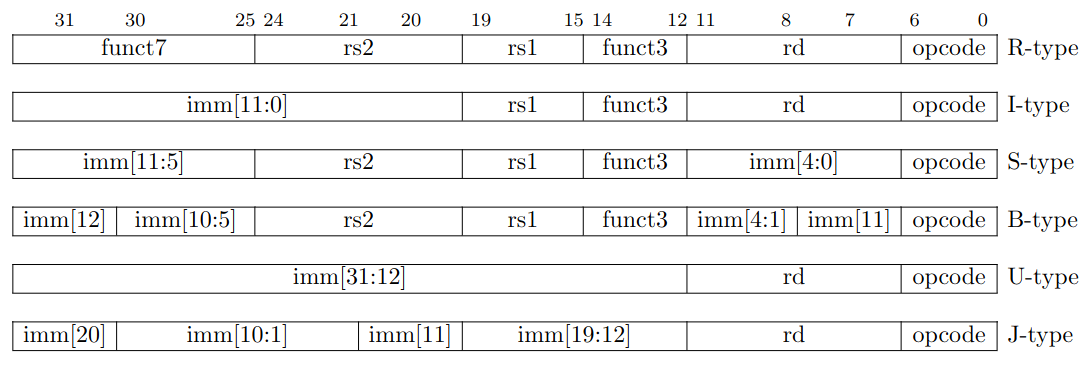
\includegraphics[width=1\linewidth]{figures/RISCV_basic_instruction_format.png}
    \caption{RISC-V instruction format}
    \label{fig:riscv_base_instruction_format}
\end{figure}

\subsection{Standard Extensions}
\begin{itemize}
    \item M refers to integer multiplication and division extension. For multiplication, there are \texttt{mul}, \texttt{mulh}, \texttt{mulhu}, \texttt{mulhsu}, and \texttt{mulw}. For division, there are \texttt{div}, \texttt{divu}, \texttt{divw}, \texttt{divuw}, \texttt{rem}, \texttt{remu}, \texttt{remw}, and \texttt{remuw}.
    
    \item A refers to atomic extension. There are \texttt{lr} (load-reserved), \texttt{sc} (store-conditional), \texttt{amoswap}, \texttt{amoadd}, \texttt{amoand}, \texttt{amoor}, \texttt{amoxor}, \texttt{amomin}, \texttt{amominu}, \texttt{amomax}, and \texttt{amomaxu}.
    
    \item C refers to compressed instructions. Around 50\%-60\% of RISC-V instructions can be compressed. This results in code size reduction of 25\%-30\%.\cite{riscv_manual} 
    
    \item F/D refer to single-precision floating point and double-precision floating point extension respectively.
    
    \item P refers to packed SIMD extension.
    
    \item V refers to vector extension.
\end{itemize}

\section{ETISS}

ETISS, which stands for Extendable Translating Instruction Set Simulator, is developed by TUM EDA chair.
As shown in Figure~\ref{fig:etiss_structure}, it is a C++ instruction set simulator based on dynamic binary translation technique. Furthermore, it features Plugin mechanism for adding new functionalities flexibly.

\begin{figure}[htbp]
    \centering{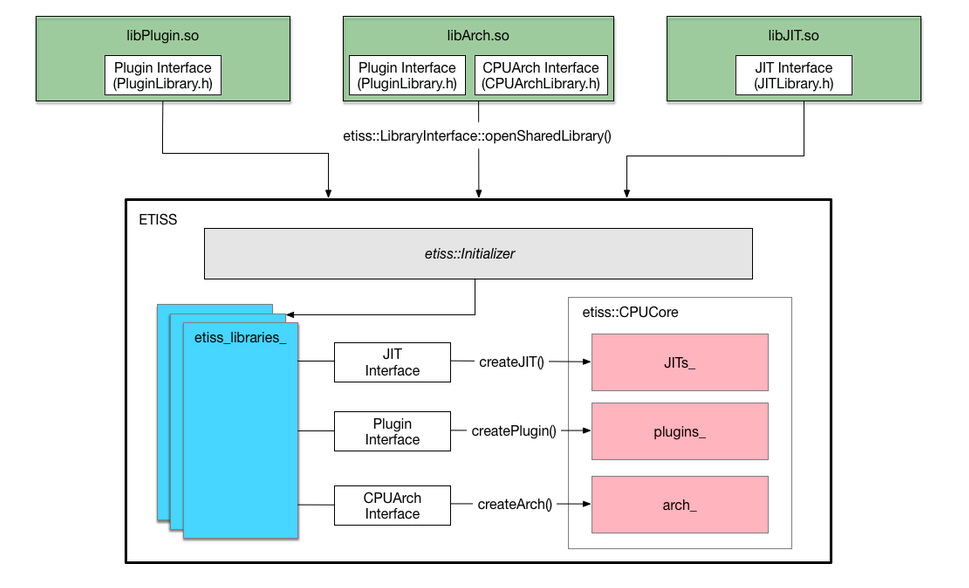
\includegraphics[scale=.4]{figures/ETISS_overview.png}}
    \caption{ETISS structure}
    \label{fig:etiss_structure}
\end{figure}

The following will describe more details on dynamic binary translation and Plugin mechanism respectively.

\subsection{Binary Translation}
Figure~\ref{fig:etiss_binary_translation} illustrates the workflow of dynamic binary translation in ETISS.
First of all, translation block is the atomic unit in binary translator. Program counter is used to check whether the corresponding translation block exists in translation cache.
If not, instructions are fetched starting from current program counter such that a new translation block is loaded. Then, the translation block is translated into C code.
The C code snippet that represents the behaviour of all instructions in a translation block is wrapped as a function in C. The function is compiled into shared library object and cached.
Whenever it is needed, it is loaded into ETISS main loop for execution. 

% Exception handling, interrupts

\begin{figure}[htbp]
    \centering{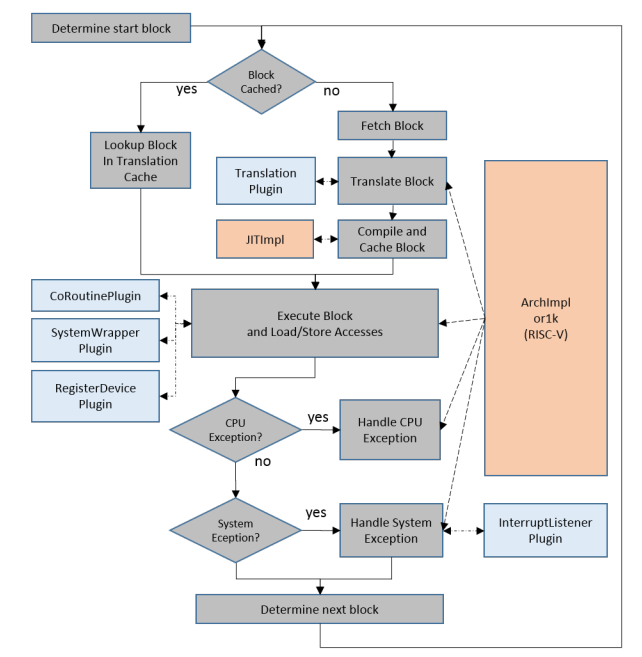
\includegraphics[scale=.45]{figures/ETISS_binary_translation.png}}
    \caption{ETISS Binary Translation}
    \label{fig:etiss_binary_translation}
\end{figure}

\subsection{Plugin Mechanism}
Plugins not only support the core binary translation process but also add functionalities to ETISS based on user's needs without hacking the core ETISS source code.
There are mainly six types of Plugins. For most of the types, an arbitrary number of Plugins can be registered.

\textbf{TranslationPlugin}: TranslationPlugins are executed before translating block. They can be used to add additional C code into translation block and to record the change of state that developers are interested in. Thus, for example, instruction tracing functionality is implemented as TranslationPlugin.

\textbf{CoroutinePlugin}: CoroutinePlugins are executed before the execution of tranlation block. They are mainly used to model closely-coupled peripherals, supporting
interrupt handling and timer functionality.

\textbf{SystemWrapperPlugin}: SystemWrapperPlugins are executed before read/write functions are called. They are mainly used to model load/store behaviours in ETISS framework.

\textbf{RegisterDevicePlugin}: RegisterDevicePlugins serve as the listeners of the architectural registers of interest. As long as register values change, they are notified for further modeling certain parts of closely-coupled peripheral functionalities.

\textbf{ISAPlugin}: One ISAPlugin is registered for each ETISS core. It defines and specifies how instructions are translated and executed in ETISS main loop, including instruction behaviour, instruction binary encoding, and register conventions.

\textbf{JITPlugin}: One JITPlugin is registered for an ETISS instance. It provides the Just-In-Time (JIT) compilation functionality, which compiles C code from translation block into shared libraries.

\section{ELF File}
ELF, which stands for Executable and Linkable Format, is the standard format for executable, relocatable, shared object, and core dump on UNIX-like operating system. The followings are the main components in ELF file.

\subsection{ELF File Header}
\label{subsec:ELF}

ELF file header contains general information of the binary and can be extracted with command line \texttt{\$readelf --header}. An example is shown in fig~\ref{fig:elf_header_example}. It starts with ELF magic number 0x7f and the "ELF" string in ASCII format. And \texttt{Type} can be \texttt{EXEC}, \texttt{REL}, \texttt{DYN}, and \texttt{CORE}. Besides, it indicates pointers to \textit{program headers} and \textit{section headers} and specifies entry point address for executable.

For RISC-V architecture, the \texttt{Flags} field is especially important since it indicates which RISC-V extensions are used and which ABIs should be respected. The layouts are shown in table~\ref{table:elf_header_flags_layout}. 

\begin{table}
    \centering
    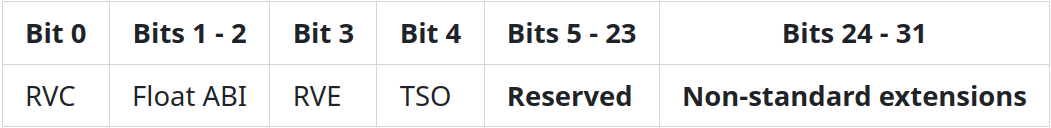
\includegraphics[width=.85\linewidth]{figures/ELF_header_flags_layout.png}
    \caption{Layout of \texttt{Flags} of RISC-V Architecture}
    \label{table:elf_header_flags_layout}
\end{table}

\begin{itemize}
    \item Bit 0 indicates whether C standard extension is used.
    \item Bits 1-2 identify four different floating point ABIs, namely \texttt{SOFT}, \texttt{SINGLE}, \texttt{DOUBLE}, and \texttt{QUAD}.
    \item Bit 3 indicates whether RVE ABI is used.
    \item Bit 4 indicates whether \textit{total store ordering} (TSO) extension is used.
\end{itemize}

\begin{figure}
    \centering
    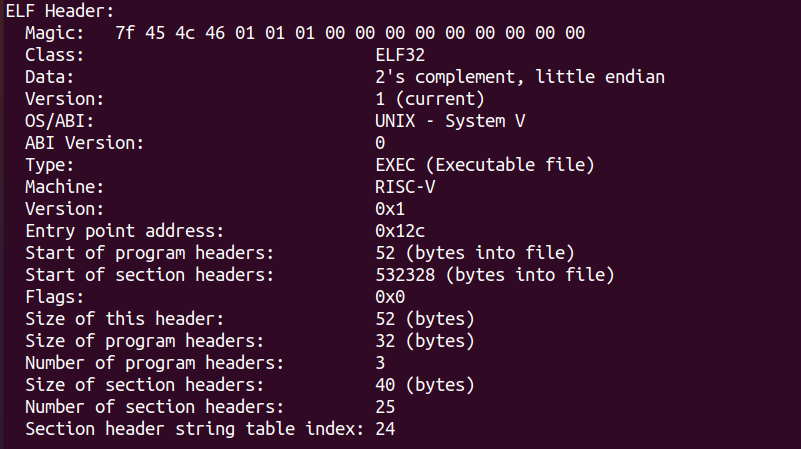
\includegraphics[width=.85\linewidth]{figures/ELF_Header.png}
    \caption{Example of ELF File Header}
    \label{fig:elf_header_example}
\end{figure}

\subsection{Sections and Segments}
ELF is versatile. For linker, sections in ELF are the source of truth. Meanwhile, segments in ELF describe how the binary is processed by loader and kernel. Being said, segments and sections are not orthogonal but interconnected. 

\subsubsection{Segments}
As shown in fig~\ref{fig:elf_program_headers_example}, there are eight fields describing each segment:

\begin{itemize}
    \item \texttt{Type} notifies operating system to load the segment if it is labeled as \texttt{LOAD}. Besides, \texttt{PHDR} means program header and \texttt{INTERP} points out the \textit{dynamic loader} for binary file.
    
    \item \texttt{Offset} refers to byte offset of the segment in ELF file. Linker and loader rely on this information to retrieve correct segment data.
    
    \item \texttt{VirtAddr} and \texttt{PhysAddr} specify where loadable segments should be placed in operating system address space.
    
    \item \texttt{FileSiz} refers to byte size of the segment in ELF.
    
    \item \texttt{MemSiz} refers to byte size of the segment in memory. If \texttt{MemSiz} is greater than \texttt{FileSize}, it means some data is zero-filled and need not be placed in ELF.

    \item \texttt{Flg} specifies permissions. \texttt{R} means readable, \texttt{W} means writable, and \texttt{X} means executable.
    
    \item \texttt{Align} specifies alignment of the segment in memory. Typically, it means the page size of operating system. In the case of fig~\ref{fig:elf_program_headers_example}, it is 4 KB. 
\end{itemize}

\begin{figure}
    \centering
    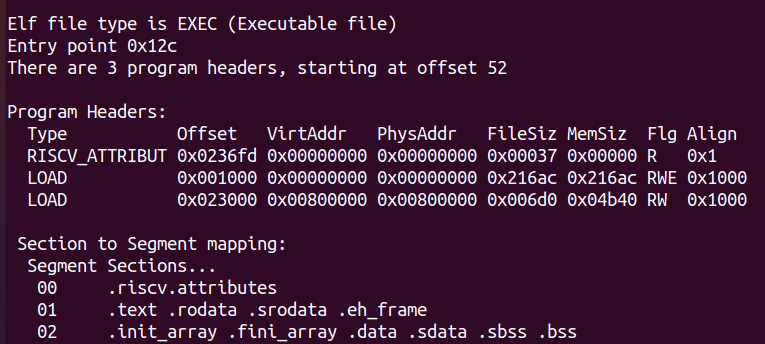
\includegraphics[width=.85\linewidth]{figures/ELF_program_header.png}
    \caption{Example of ELF File Program Header}
    \label{fig:elf_program_headers_example}
\end{figure}

\subsubsection{Sections}

\begin{itemize}
    \item \texttt{.text} is where executable code locates.
    \item \texttt{.rodata} stores read-only data.
    \item \texttt{.data} stores initialized and writable data.
    \item \texttt{.bss} stores zero-initialized and writable data.
    \item \texttt{.symtab} refers to symbol table that stores the mapping between symbols and their locations in ELF, as shown in fig~\ref{fig:elf_symbol_table}. As section~\ref{subsec: elf_info_extraction} will give more details, it is useful for extracting mapping of functions to program counter ranges.
    \item \texttt{.debug\_info} stores main debug information in DWARF format. It appears only when the binary is compiled with \texttt{-g} option.
    \item \texttt{.debug\_line} stores the mapping between program counter and source code line. It also appears only when the binary is compiled with \texttt{-g} option.
\end{itemize}

\subsection{DWARF Format}
DWARF format is the most common debugging format. It is of great importance since GNU debugger (GDB) and LLVM debugger (LLDB) heavily rely on information stored in DWARF-related ELF sections.

DWARF distills information about application program into a tree structure. The tree structure contains multiple \textbf{debugging information entries} (DIEs), which is available by giving the command line \texttt{\$readelf --debug-dump=info <elf file>}. A DIE may have parent DIE, siblings DIEs, or children DIEs. Each DIE contains a \textit{tag} and several \textit{attributes}. \textit{Tag} is the label of a DIE. It can be scope-related, object-related, or type-related. 

\begin{itemize}
    \item Common scope-related \textit{tags}: \textit{compile\_unit}, \textit{namespace}, \textit{subprogram}, \textit{inline\_subroutine},  \textit{label}, \textit{call\_site}, and \textit{lexical\_block} 
    
    \item Common object-related \textit{tags}: \textit{variable} and \textit{formal\_parameter}

    \item Common type-related \textit{tags}: \textit{base\_type}, \textit{typedef}, \textit{array\_type}, \textit{structure\_type}, \textit{union\_type}, \textit{class\_type}, \textit{enumeration\_type}, \textit{subroutine\_type}, \textit{string\_type}, and \textit{subrange\_type}.
\end{itemize}

As for \texttt{attributes}, they may contain constants, variables, or reference to another DIE.~\cite{dwarf}. Several examples are as follows:

\begin{itemize}
    \item \textit{DW\_TAG\_compile\_unit}: As shown in \ref{fig:dwarf_compile_unit}, there are \textit{producer}, \textit{language}, \textit{name}, \textit{comp\_dir}, \textit{low\_pc}, \textit{high\_pc}, \textit{stmt\_list}.
    
    \item \textit{DW\_TAG\_subprogram}: As shown in \ref{fig:dwarf_subprogram}, there are \textit{external}, \textit{name}, \textit{decl\_file}, \textit{decl\_line}, \textit{decl\_column}, \textit{low\_pc}, \textit{high\_pc}, \textit{frame\_base}, \textit{sibling}.

    \item \textit{DW\_TAG\_inlined\_subroutine}: As shown in \ref{fig:dwarf_inlined_subroutine}, there are \textit{abstract\_origin}, \textit{entry\_pc}, \textit{ranges}, \textit{call\_file}, \textit{call\_line}, \textit{call\_column}.

    \item \textit{DW\_TAG\_base\_type}: As shown in \ref{fig:dwarf_base_type}, there are \textit{byte\_size}, \textit{encoding}, and \textit{name}.
\end{itemize}

\begin{figure}
    \centering
    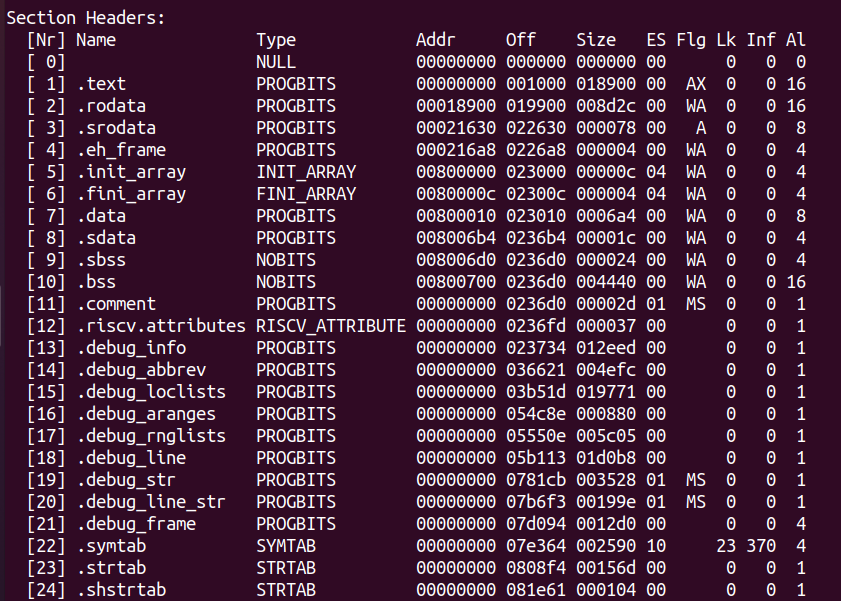
\includegraphics[width=.85\linewidth]{figures/ELF_section_header.png}
    \caption{Example of ELF File Section Header}
    \label{fig:elf_section_headers_example}
\end{figure}

\begin{figure}
    \centering
    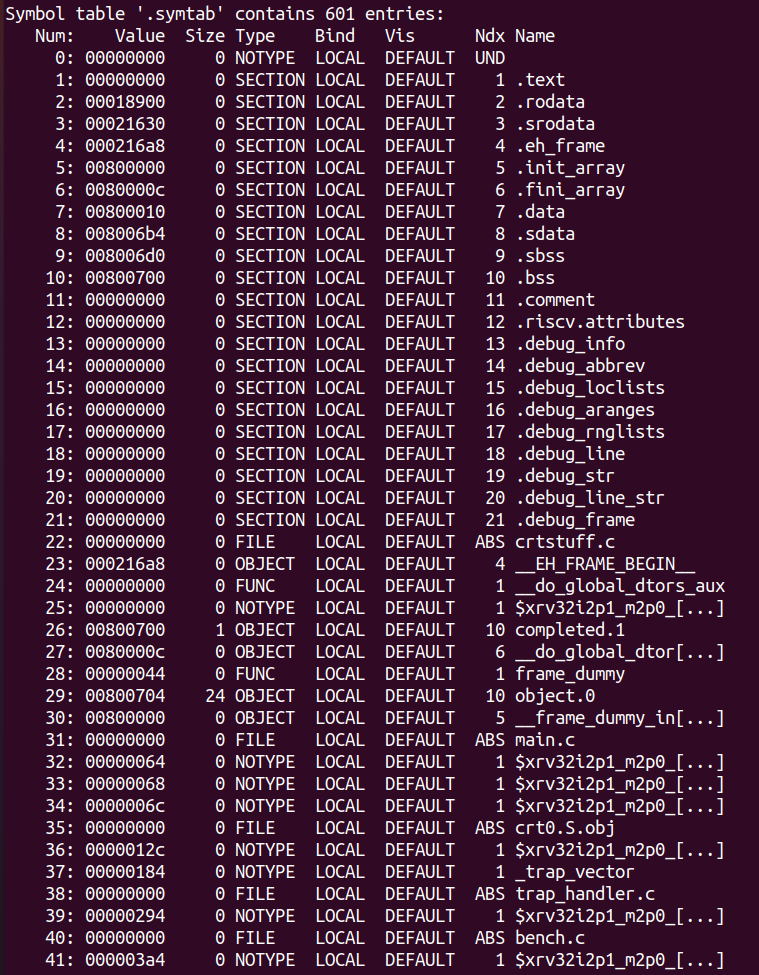
\includegraphics[width=.8\linewidth]{figures/ELF_symtab.png}
    \caption{Example of ELF file symbol table}
    \label{fig:elf_symbol_table}
\end{figure}

\begin{figure}
    \centering
    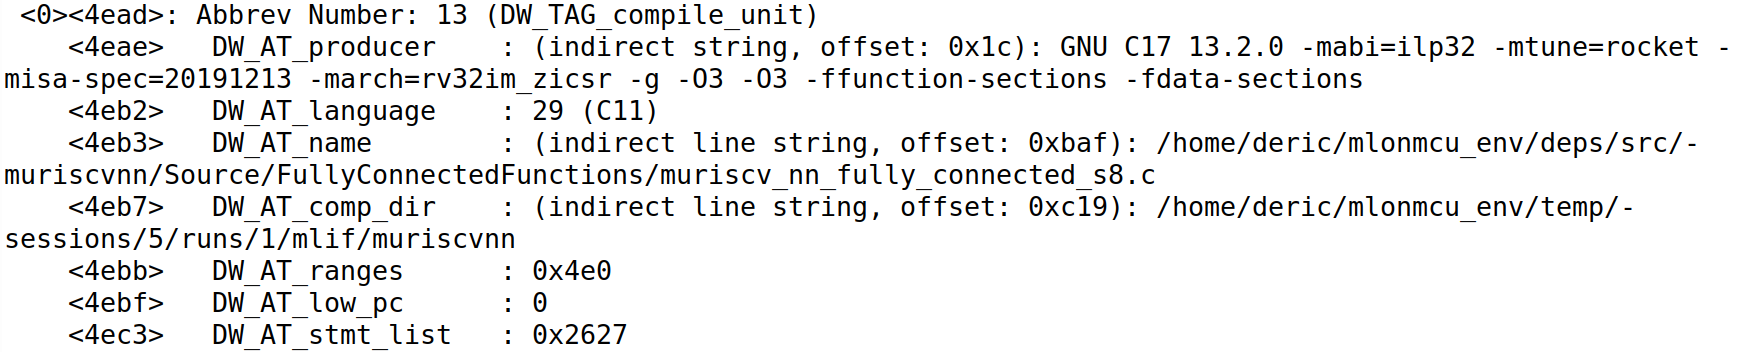
\includegraphics[width=.9\linewidth]{figures/DWARF_compile_unit.png}
    \caption{Example of DWARF compile unit}
    \label{fig:dwarf_compile_unit}
\end{figure}

\begin{figure}
    \centering
    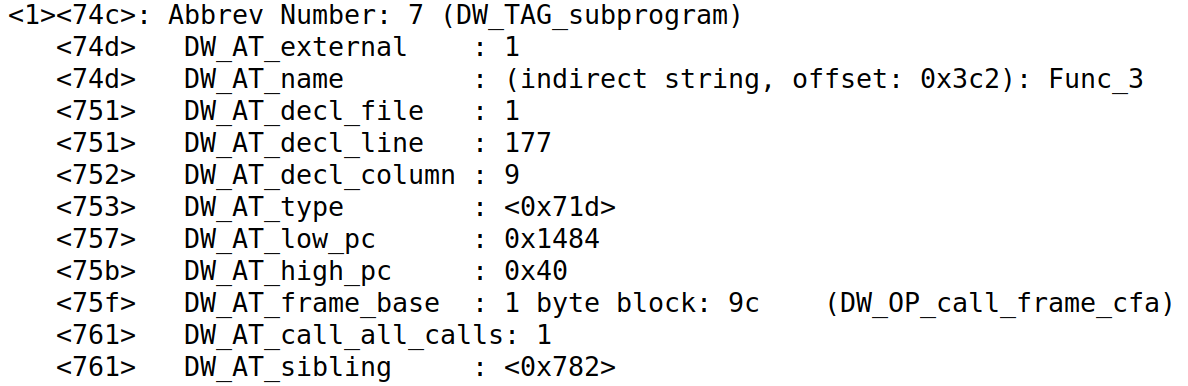
\includegraphics[width=.75\linewidth]{figures/DWARF_subprogram.png}
    \caption{Example of DWARF subprogram}
    \label{fig:dwarf_subprogram}
\end{figure}

\begin{figure}
    \centering
    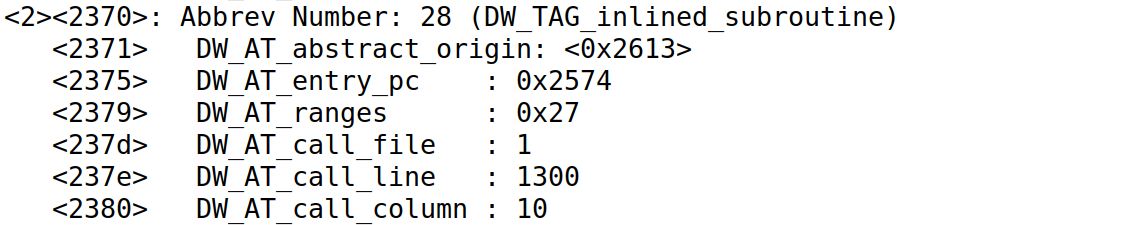
\includegraphics[width=.75\linewidth]{figures/DWARF_inlined_subroutine.png}
    \caption{Example of DWARF inlined subroutine}
    \label{fig:dwarf_inlined_subroutine}
\end{figure}

\begin{figure}
    \centering
    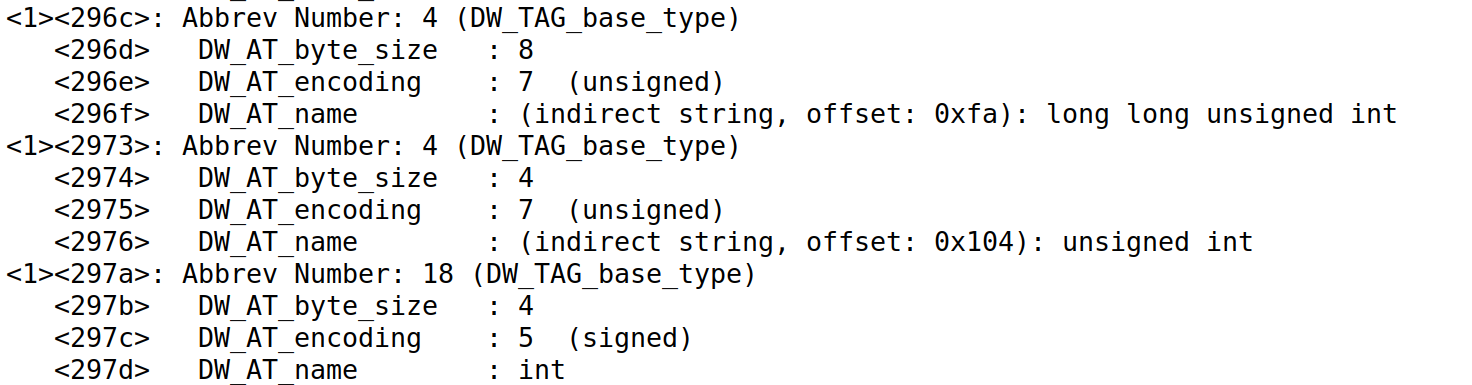
\includegraphics[width=.75\linewidth]{figures/DWARF_base_type.png}
    \caption{Example of DWARF base type}
    \label{fig:dwarf_base_type}
\end{figure}

\subsection{Line Number Table}
\label{subsec:line_table}

Line number table contains the mapping between program counter and corresponding source code. It is stored in ELF \texttt{.debug\_line} section, which is available by giving command line \texttt{\$readelf --debug-dump=line <elf file>}. There are three main components in line number table, namely \textit{directory table}, \textit{file name table}, and \textit{line number statement}.

\begin{itemize}
    \item \textit{Directory table and File name table}: As shown in \ref{fig:dwarf_debug_prologue}, \texttt{File name table} together with \texttt{directory table} clearly show the files and their indices in each directory.
    
    \item \textit{Line number statement}: 
\end{itemize}


\begin{figure}
    \centering
    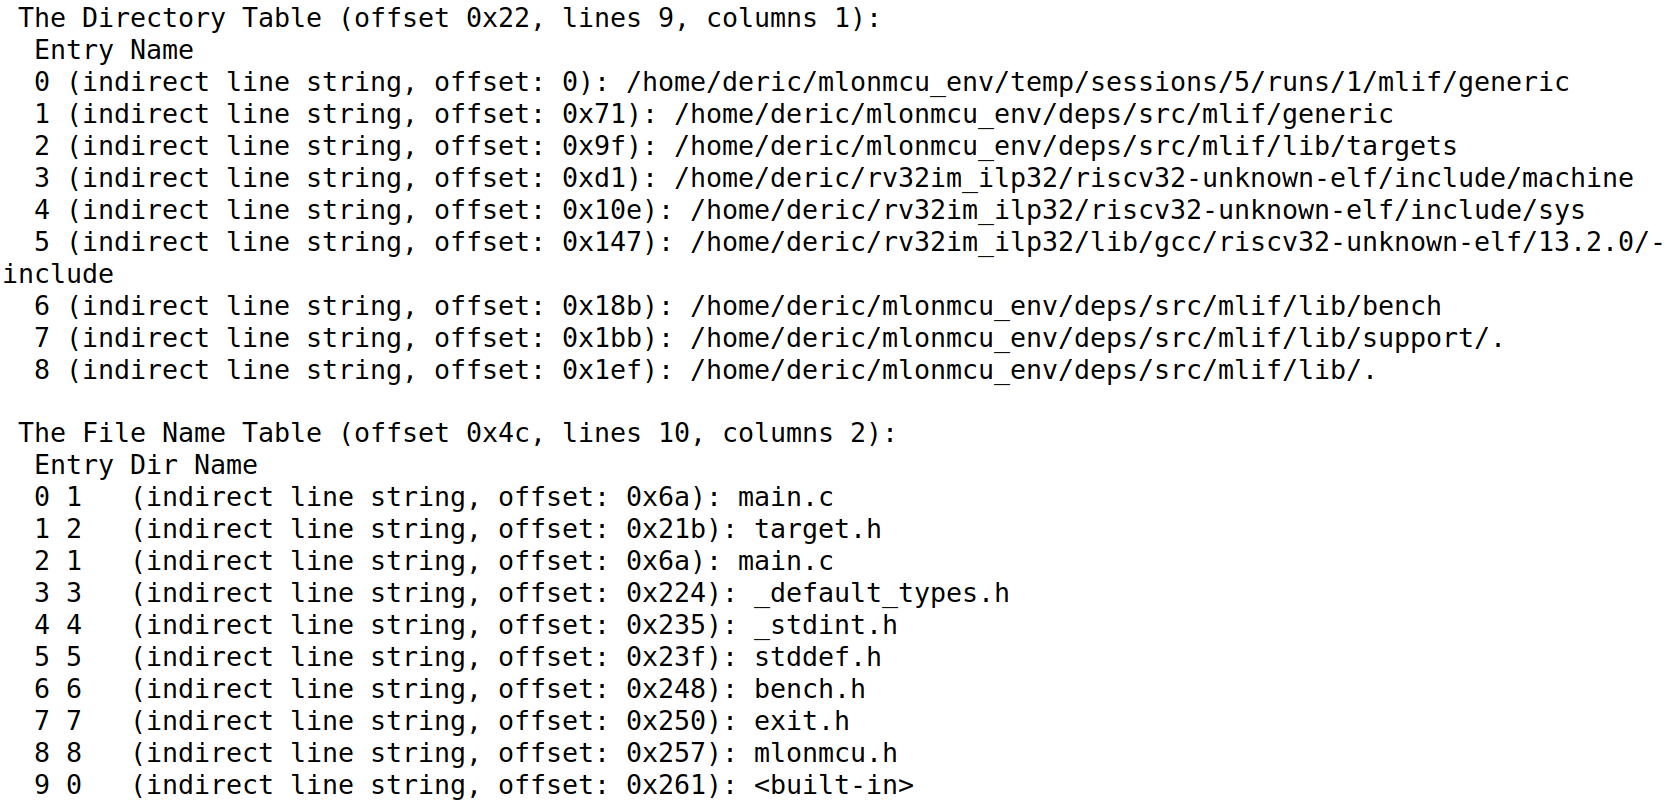
\includegraphics[width=.95\linewidth]{figures/DWARF_debug_prologue.png}
    \caption{Example of DWARF directory table and file name table}
    \label{fig:dwarf_debug_prologue}
\end{figure}

\begin{figure}
    \centering
    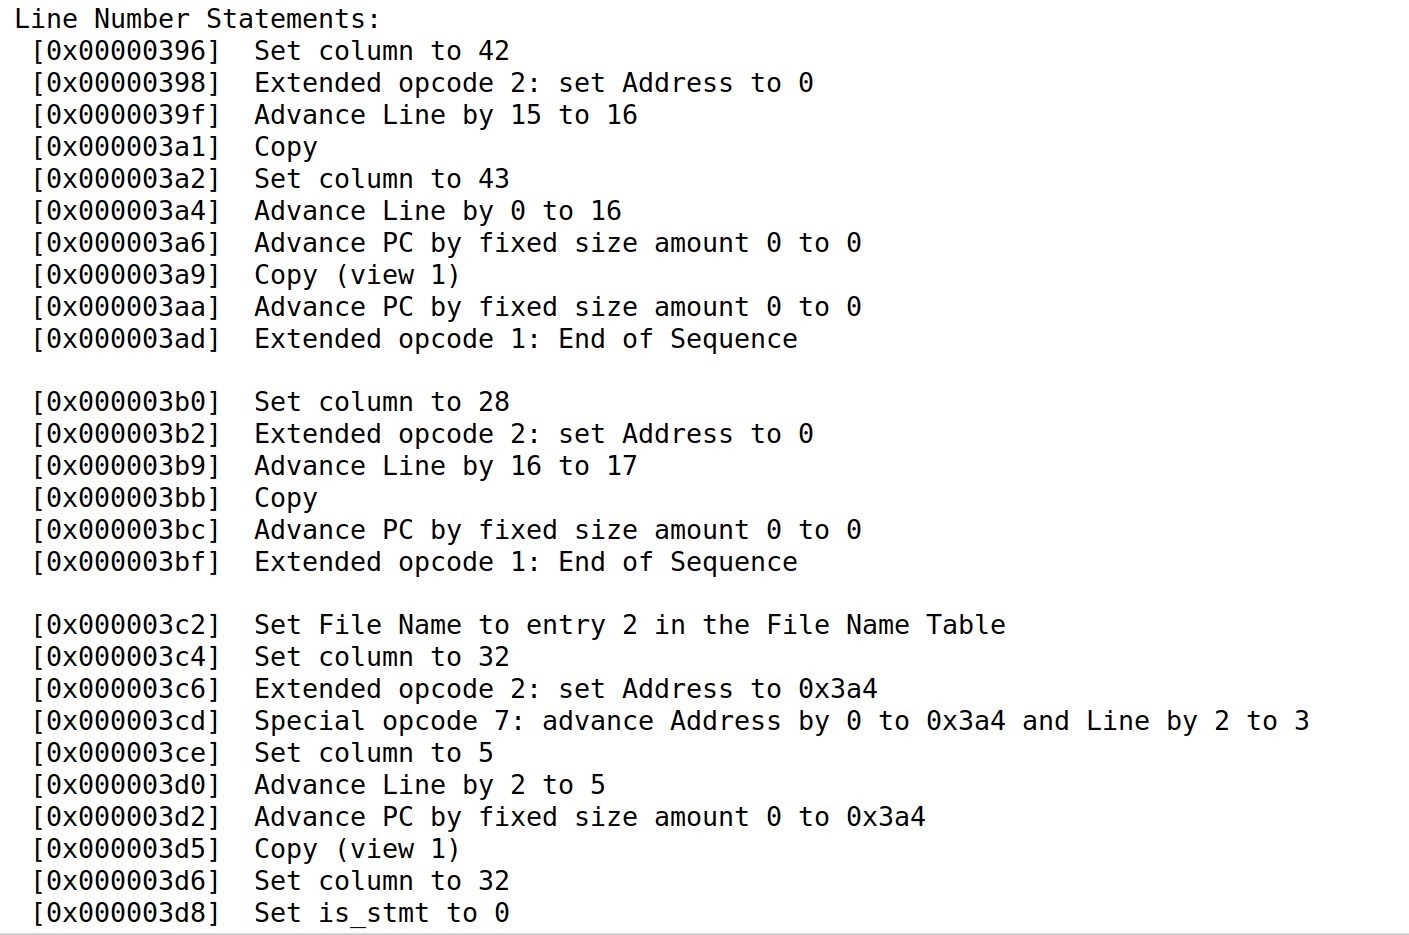
\includegraphics[width=.85\linewidth]{figures/DWARF_debug_main.png}
    \caption{Example of DWARF line number statement}
    \label{fig:dwarf_debug_main}
\end{figure}


\section{Machine Learning Deployment}
Open source deep learning frameworks, such as PyTorch and Tensorflow, are widely known to end users. In contrast, the underlying software stacks that deploy deep learning workloads on diverse hardware backends are less known but extremely crucial. To be more concrete, it is the so-called machine learning compiler that deals with the huge gap between high-level computational graph and binary executable. The following are two widely-used machine learning compiler frameworks.

\begin{figure}
    \centering
    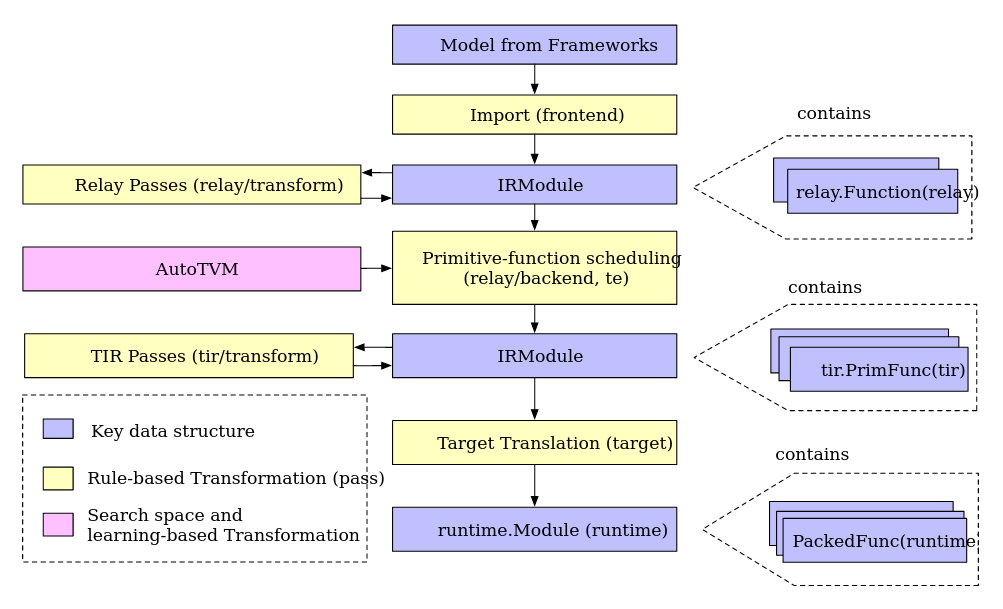
\includegraphics[width=1\linewidth]{figures/TVM_compilation_flow.png}
    \caption{Compilation Flow of TVM}
    \label{fig:tvm_compilation_flow}
\end{figure}

\subsection{TVM}
TVM was developed by a research group at the University of Washington and has evolved into one of the most popular open-source machine learning compiler frameworks. Figure~\ref{fig:tvm_compilation_flow} clearly shows the compilation flow of TVM and its key data structures.

Regarding key data structures, there are two types of intermediate representation (IR), Relay IR and Tensor IR. Relay IR is a high-level functional frontend IR that aims to represent deep learning workloads as computational graphs. On the other hand, Tensor IR is a low-level backend IR for code generation. It represents detailed information about target-specific optimizations on loop structures, memory access patterns, and vector/tensor instructions.

The compilation flow is described in the following.
\begin{enumerate}
    \item It starts with the import of deep learning models of various types and from different frameworks, such as onnx, Tensorflow, PyTorch, and TFLite. The input model is transformed and stored as Relay IRModule.
    \item A collection of Relay passes are responsible for graph-level optimizations. Graph-level optimizations typically include constant-folding, shape inference, canonicalization, dead code elimination, operator fusion and data layout transformation. \textit{Constant-folding} pass identifies graph nodes, of which inputs and outputs are known, precomputes them, then propagates constants through the graph. \textit{Shape inference} pass aims to convert dynamic shapes into static shapes by inferring the inputs and outputs of graph nodes. \textit{Operator fusions} pass aims to fuse multiple operators, minimizing unnecessary data transfer. The predefined seven types of operator, namely elementwise, broadcasting, injective, communicative reduction, complex, tuple, opaque, build the basics of the algorithm.
    \textit{Data layout transformation} pass transforms data layouts into what hardware backend expects or prefers.
    \item AutoTVM is responsible for optimizations that require design-space explorations, such as loop tiling, memory latency hiding, tensorization and many more. In general, the goal is to increase data reuse on the specified hardware backend. However, the fact that there are more and more new machine learning hardware makes the approach of handcrafting each target's characteristics unrealistic. The optimizations in AutoTVM are led by search-based or learning-based algorithms.
    \item 
    
\end{enumerate}

\subsection{MLIR}
MLIR was introduced by Chris Lattner at Google. It is widely used in different domains, including not only machine learning deployment but also quantum computing and query compilation. The main features of MLIR are (1) the flexibility to perform progressive lowering and optimizations at unfixed levels of abstraction, (2) the flexibility to define custom intermediate representation, which is called dialect, and (3) the flexibility to define rewrite patterns in a declarative way.

\subsubsection{IR Design}
An example in figure~\ref{fig:mlir_ir_design} provides an overview of IR design in MLIR. The main components of IR design are dialect, operation, attribute, region, and location information.

\begin{itemize}
    \item \textit{Operation} is the atomic entity in IR. The operation shown in figure~\ref{fig:mlir_ir_design} is \textit{conv2d}. It takes operands \textit{\%input}, \textit{\%filter}, and \textit{\%bias} with types \textit{tensor<1x225x225x3xf32>}, \textit{tensor<32x3x3x3xf32>}, and \textit{tensor<32xf32>} respectively. An operation can have one or more outputs. In this case, it returns \textit{\%0} with type \textit{\%tensor<1x112x112x32xf32>}.
    \item \textit{Attribute} represents compile-time static information of an operation instance. For \textit{conv2d} operation instance in figure~\ref{fig:mlir_ir_design}, attributes are the brace-enclosed key value pairs \textit{\{dilation = [1, 1], pad = [0, 0, 0, 0], stride = [2, 2]\}}. They are kept as a dictionary from string names to underlying values by operation instance. Besides, all attributes are typed.
    \item \textit{Region} enables nested structure inside operation. As illustrated in figure~\ref{fig:mlir_ir_region}, The top-level \textit{for} operation contains a region, where another \textit{for} operation and a terminator \textit{yield} operation exist. Being said, region contains a list of operations, which may also contain regions. This is especially useful for defining structure such as control flow.
    \item \textit{Location information} preserves the source information during the lowering and optimizations process. It is useful for debugging and also for understanding how lowering and optimizations actually work on each operation. 
    \item \textit{Type} is strictly attached to each value in MLIR. There are standard types, including integer, floating point, tensor, vector, memref, tuple and many more. Besides, MLIR type system is extensible to custom dialects and foreign dialects, such as LLVM IR dialect and SPIR-V dialect.
\end{itemize}

Dialect is the container for the above components. It provides granularity for reasoning about the level of abstraction. Common MLIR dialects are shown in figure~\ref{fig:mlir_dialects_overview}. From a high level perspective, MLIR dialects can be categorized through \textit{tensor/buffer} and \textit{payload/structure} axes. \textit{Tensor/buffer} axis indicates whether the dialect of interest mainly deals with \textit{tensor} or \textit{buffer}. The former is typically seen in ML frameworks, whereas the latter is much more relevant to actual memory access. As a result, bufferization is the core of progressive lowering in MLIR, meaning that high-level dialects, such as \textit{onnx-mlir}, \textit{torch-mlir} and \textit{tosa}, are progressively bufferized into lower-level dialects, including \textit{linalg},\textit{memref}, and \textit{arith}. \textit{Payload/structure} axis distinguishes between \textit{what} or \textit{how} computations should be performed. For example, tosa dialect supports common machine learning operators as its operations. However, it doesn't specify how those operators should actually be performed. On the other hand, linalg dialect represents how computations are performed on the structure of interest.

\subsubsection{IR Infrastructure}

IR infrastructure is the core basis that supports IR design. It provides not only great extensiblity to custom dialect design, but also simplifies the usage of MLIR main functionalities from user perspective.

\begin{itemize}
    \item \textit{Operation Descriptions} is supported through TableGen in MLIR. Compared to the usage of C++ template, it is much more intuitive regarding programability, as shown in figure~\ref{fig:mlir_ods}. Moreover, the table-driven manner keeps all the information about the operation of interest in one place such that helper functions generation, verification and analysis for can be done easily.
    
    \item \textit{Rewrite Patterns Declaration} is crucial in MLIR since optimization and lowering rely on this mechanism. The PDL language (PDLL) is a frontend declarative DSL dedicated to pattern matching and rewrite as shown in figure~\ref{fig:mlir_pdll}.
    
    \item \textit{Verifiers} enforce the structure and semantics of IR to be aligned with specification. For example, types should match and terminator operation should exist at the end of each region.
\end{itemize}

\begin{figure}
    \centering
    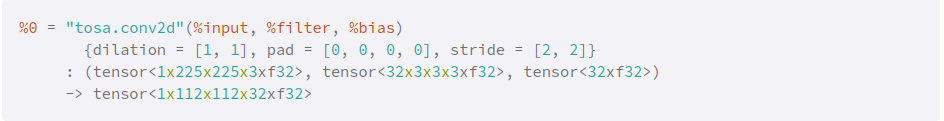
\includegraphics[width=1.\linewidth]{figures/MLIR_IR_design.png}
    \caption{MLIR IR Example}
    \label{fig:mlir_ir_design}
\end{figure}

\begin{figure}
    \centering
    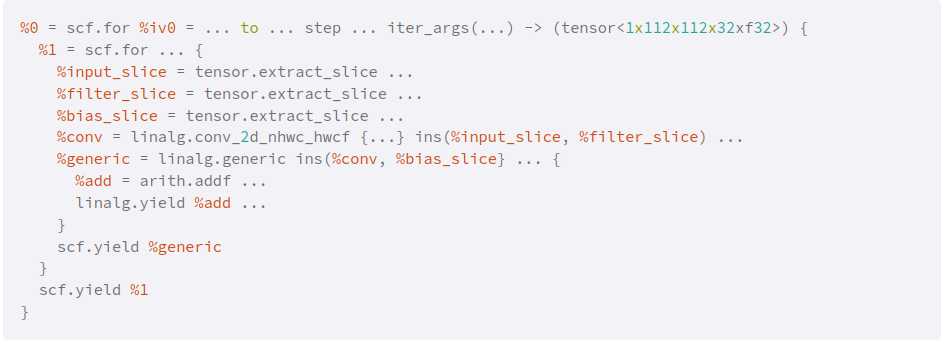
\includegraphics[width=1.\linewidth]{figures/MLIR_IR_region.png}
    \caption{Region in MLIR IR}
    \label{fig:mlir_ir_region}
\end{figure}

\begin{figure}
    \centering
    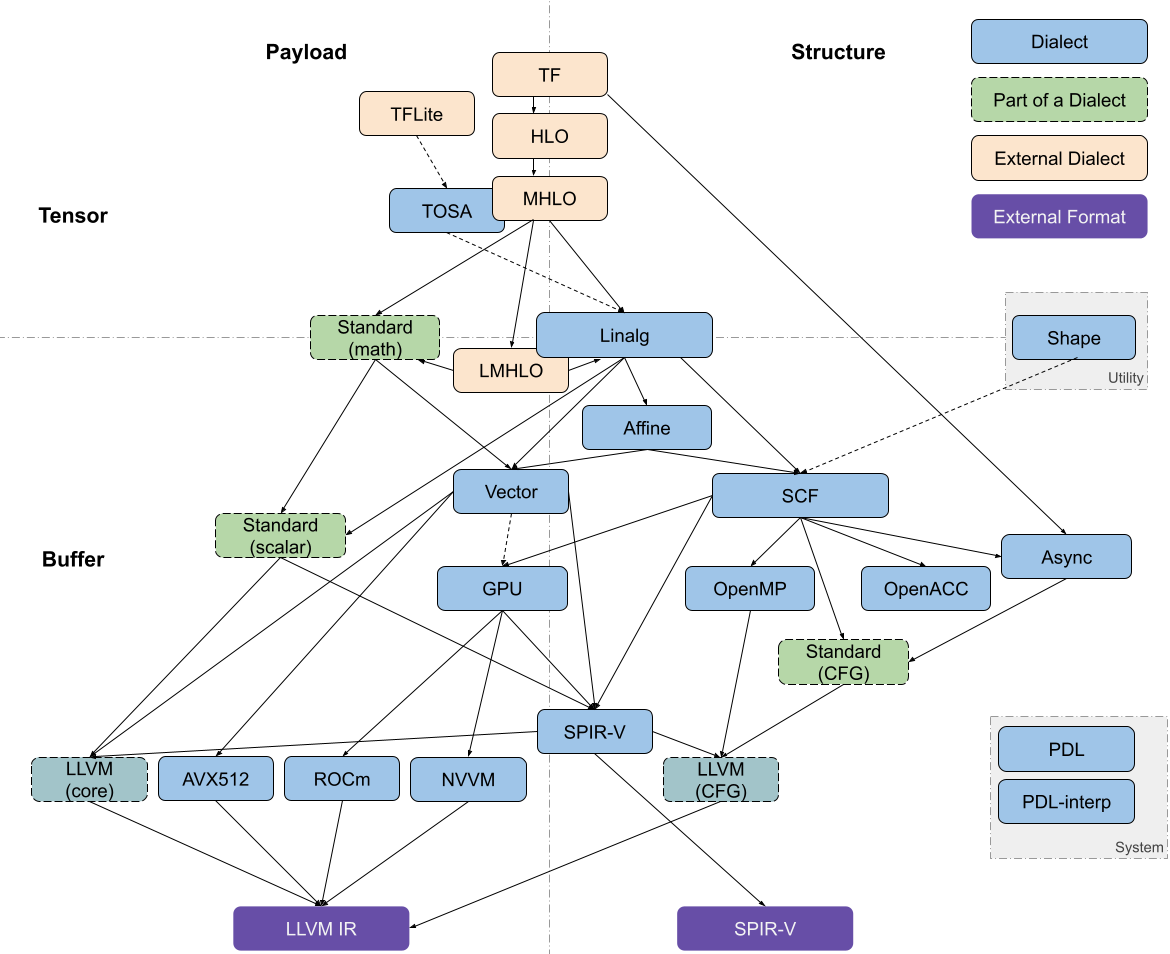
\includegraphics[width=0.8\linewidth]{figures/MLIR_dialect_overview.png}
    \caption{Overview of MLIR Dialects}
    \label{fig:mlir_dialects_overview}
\end{figure}

\begin{figure}
    \centering
    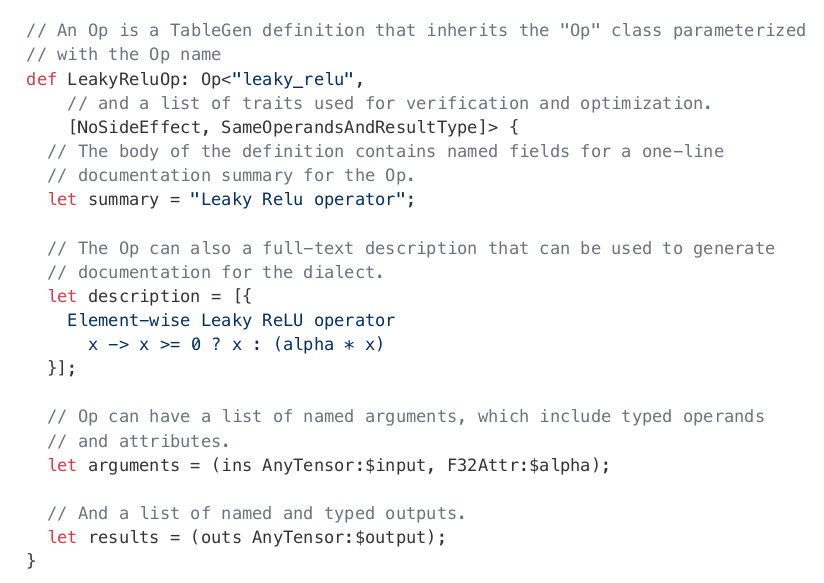
\includegraphics[width=0.8\linewidth]{figures/MLIR_ODS.png}
    \caption{Example of Defining Custom Operation with ODS}
    \label{fig:mlir_ods}
\end{figure}

\begin{figure}
    \centering
    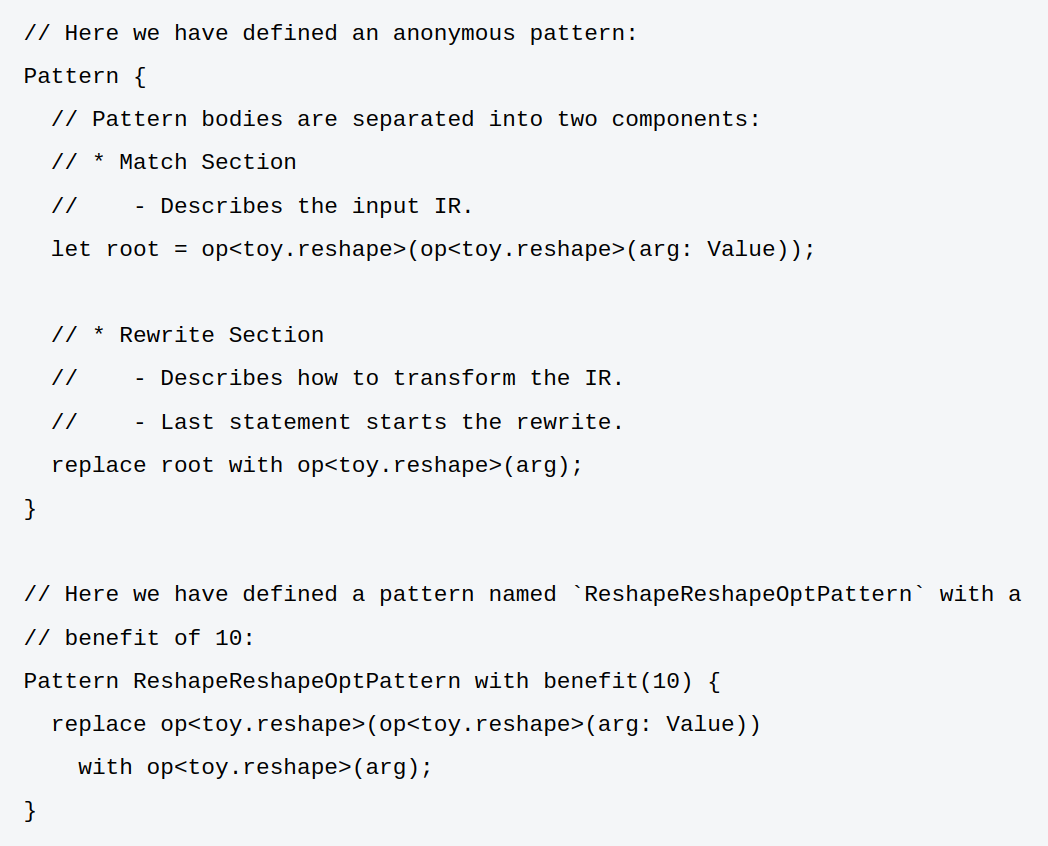
\includegraphics[width=0.6\linewidth]{figures/MLIR_PDLL.png}
    \caption{Example of Declaring Rewrite Patterns with MLIR PDLL}
    \label{fig:mlir_pdll}
\end{figure}

\section{Valgrind}
Valgrind is a widespread software tool for profiling and debugging. To put it in a simple way, it is a virtual machine. The \textit{core} part includes a just-in-time (JIT) compiler and some reimplementations of glibc that deal with signal handling and thread scheduling, whereas the \textit{skin} part is similar to plugin. Custom \textit{skins} can be developed to supervise the aspect of program execution of interest, as long as the \textit{core/skin} interface is respected. Some widely known \textit{skins} are \textit{Memcheck}, \textit{Helgrind}, \textit{ThreadSanitizer}, \textit{Massif}, \textit{Cachegrind}, and \textit{Callgrind}.

\subsection{Core}

\begin{itemize}
    \item JIT compilation: Valgrind internals use \textit{Ucode} as intermediate representation. During binary translation, each basic block is (1) translated to \textit{UCode} format~\ref{fig:valgrind_UCode}, (2) optimized, (3) added with instrumentation, then (3) translated back to x86 instructions~\ref{fig:valgrind_UCode_back}.
    \item Signal Handling: Valgrind intercepts system calls related to signal handling. This way, it can not only fully control application program, but can also mask signals of interest for \textit{skins}.
    \item Thread Scheduling: The \textit{core} has its implementation of pthread functionality. It fully controls thread scheduling, preemption, and synchronization of application program.
\end{itemize}

\begin{figure}
    \centering
    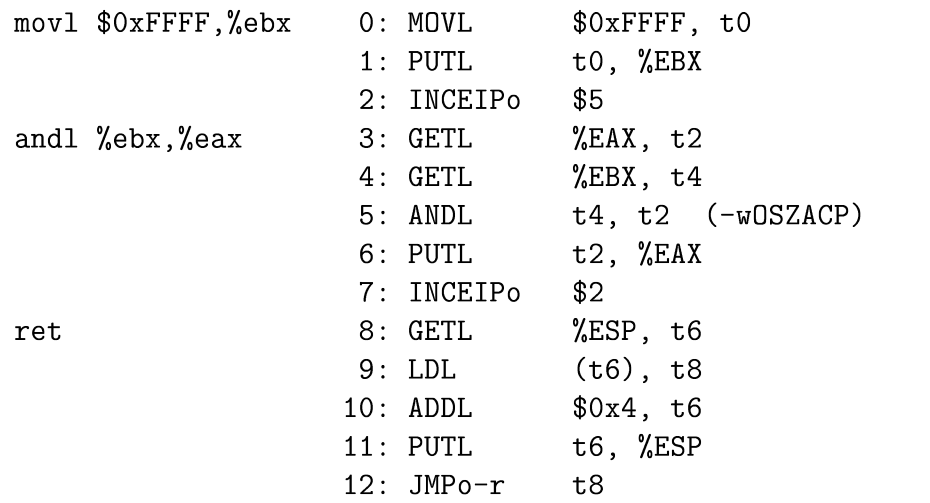
\includegraphics[width=0.55\linewidth]{figures/Valgrind_UCode.png}
    \caption{Instructions are converted to UCode format\cite{valgrind}}
    \label{fig:valgrind_UCode}
\end{figure}

\begin{figure}
    \centering
    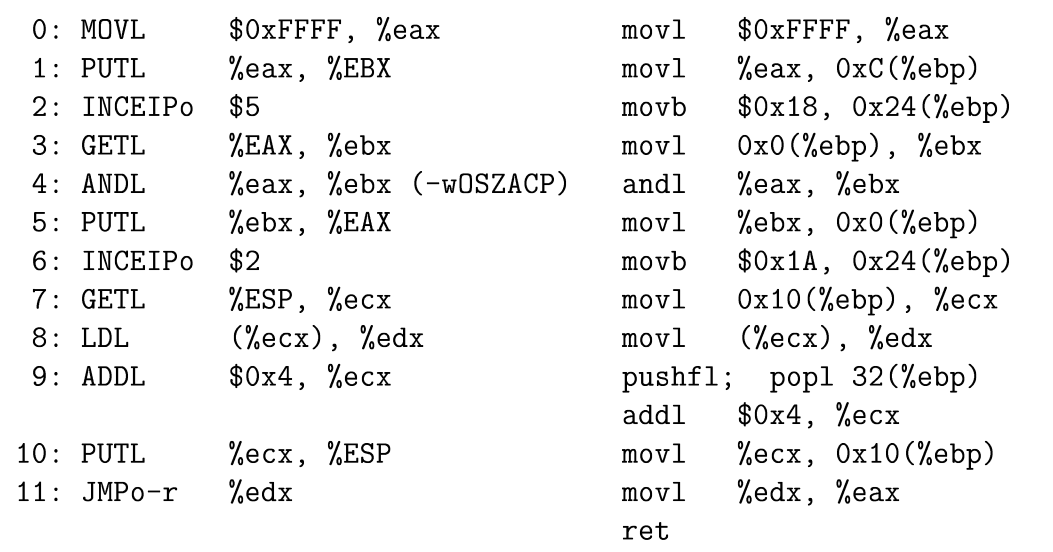
\includegraphics[width=0.55\linewidth]{figures/Valgrind_UCode_2.png}
    \caption{Instructions are converted back to x86 format\cite{valgrind}}
    \label{fig:valgrind_UCode_back}
\end{figure}

\subsection{Core/Skin Interface}
Core/skin interface specifies the APIs for users to develop their own \textit{skins}. Concretely, \textit{vgSkin\_pre\_clo\_init()}, \textit{vgSkin\_post\_clo\_init()}, \textit{vgSkin\_instrument()}, and \textit{vgSkin\_fini()} are the necessary functions of a \textit{skin}. In addition, there are extra structure fields in a \textit{skin} specifying the \textit{core} services, such as error handling, that it wants to subscribe and the events happening in the \textit{core}, such as memory allocation, that it wants to observe. In a nutshell, the design of core/skin interface provides great modularity and extensibility.

\subsection{Common \textit{Skins}}
\label{subsec:callgrind}

\begin{itemize}
    \item \textit{Memcheck} is a memory error detection tool for C/C++ applications, which is capable of reporting memory leaks and illegal memory access in details. This is achieved by maintaining the shadow memory. It represents the real memory with additional \textit{valid-value} and \textit{valid-address} states for each bit. During read/write access or memory allocation, these states are modified accordingly and consulted for errors.
    
    \item \textit{Helgrind} is a thread error detection tool. It is capable of detecting misuses of pthreads API, inconsistent lock orderings, and data races. This is achieved by using happens-before analysis~\cite{happens-before-relation} and lockset algorithm~\cite{lockset-algorithm}. And it turns out that false alarm is part of its nature.
    
    \item \textit{DRD} is also a thread error detection tool. Compared to \textit{Helgrind}, it produces more precise results at the cost of more performance overheads. This is achieved by using vector clocks~\cite{vector-clocks} instead of lockset algorithm.
    
    \item \textit{Massif} is a heap profiler. It is capable of reporting the amount of heap memory used by application program over time. This is achieved by intercepting and tracking \texttt{malloc}, \texttt{free}, \texttt{calloc}, and \texttt{realloc}. In addition, there is a standalone tool Massif-Visualizer for interactive visualization.
    
    \item \textit{Cachegrind} is a memory profiler. It is capable of simulating cache behaviour and branch prediction behaviour and reporting cache utilization, cache hits, and cache misses. This is achieved by maintaining metadata in \textit{global cache state}, \textit{cost center table}, and \textit{instr-info table}~\cite{cachegrind}.
    
    \item \textit{Callgrind} is a performance profiler. It includes all cache simulation features of \textit{cachegrind} and has call graph analysis functionality additionally. Besides, there is a powerful graphical tool \textit{Kcachegrind} for visualizing generated data interactively.
    
\end{itemize}

\subsection{Kcachegrind}
\label{subsec:kcachegrind}

As mentioned in \ref{subsec:callgrind}, \textit{Kcachegrind} is the GUI for callgrind. The main features of \textit{Kcachegrind} are as follow:

\begin{itemize}
    \item \textbf{Multiple Event Types}: \textit{Kcachegrind} visualizes all event types that \textit{callgrind} supports and enables switching between those events at ease. An example is shown in \ref{fig:kcachegrind_caller_callee}.
    
    \item \textbf{Interactive Call Graph}: Call graph is visualized in \textit{Kcachegrind} in an interactive way. Namely, users can not only click on nodes and edges for detailed information, but also use filter to focus on functions of interest. Fig \ref{fig:kcachegrind_treemaps_and_callgraphs} provides an example.
    
    \item \textbf{Source Code/Assembly Annotations}: Metrics of specific event for each line of source code and assembly are annotated right next to each of them. This way, users know, for examples caller-callee relations at the granularity of instruction level or loop structures, without any effort. Fig \ref{fig:kcachegrind_pos_annotations} is an example.
\end{itemize}

\begin{figure}
    \centering
    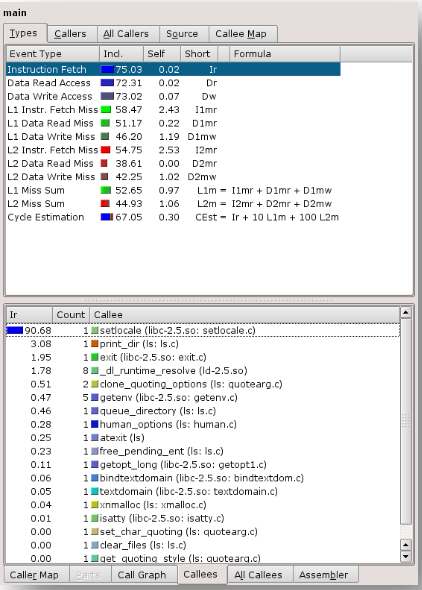
\includegraphics[width=0.65\linewidth]{figures/kcachegrind_caller_callee.png}
    \caption{Lists of event types and callers/callees in Kcachegrind~\cite{kcachegrind}}
    \label{fig:kcachegrind_caller_callee}
\end{figure}

\begin{figure}
    \centering
    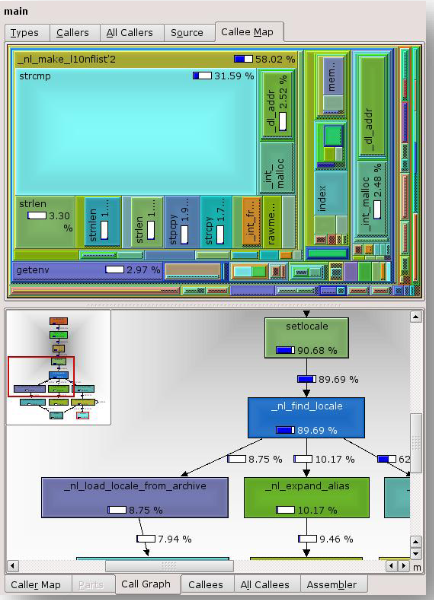
\includegraphics[width=0.65\linewidth]{figures/kcachegrind_callgraph.png}
    \caption{Treemaps and callgraphs in Kcachegrind~\cite{kcachegrind}}
    \label{fig:kcachegrind_treemaps_and_callgraphs}
\end{figure}

\begin{figure}
    \centering
    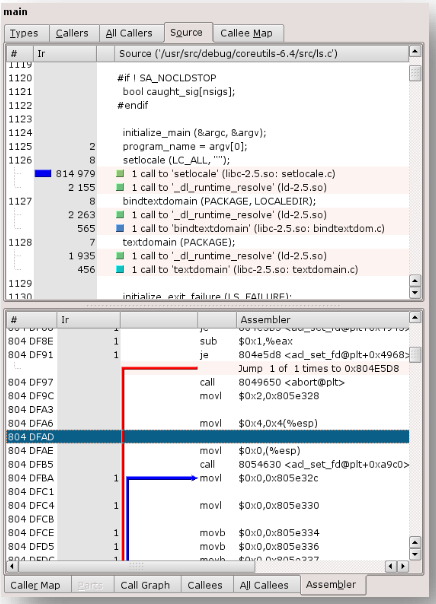
\includegraphics[width=0.65\linewidth]{figures/kcachegrind_pos_annotation.png}
    \caption{Position annotations in Kcachegrind~\cite{kcachegrind}}
    \label{fig:kcachegrind_pos_annotations}
\end{figure}